\section{LCD}
In dieser Aufgabe wirst du dich mit dem LCD beschäftigen.
Zu allererst bekommst du eine kleine Einführung in die Funktionsweise.
Darauffolgend wirst du ein paar kleine Aufgaben gestellt bekommen, um dich mit der Programmierung des Displays zurecht zu finden.

\subsection*{Einführung LCD}
Die Ansteuerung des LCD erfolgt über Pins mit festgelegten Funktionen.
Zur Vereinfachung wurden bereits im Projekt für diese Aufgabe Definitionen vorgegeben, sodass die Pins über einfache Namen angesteuert werden können. Die Namen entsprechen den Pins, wie sie im Datenblatt (\url{https://github.com/Echtzeitsysteme/tud-cpp-exercises/blob/master/doc/Display_AV128641YFBY-WSV.pdf}) ab Seite 10 zu finden sind.

\begin{center}
	\begin{tabular}{l|l|l}
		\toprule
		\textbf{Name} & \textbf{Funktion} & \textbf{Pin/Port} \\ 
		\midrule
		LCD\_PORT\_DB & Datenbus (DB0 - DB7) & P01 \\ 
		LCD\_PIN\_DI & Data (1) / Instruction (0) & P02\_0 \\ 
		LCD\_PIN\_RW & Read (1) / Write (0) & P02\_1 \\ 
		LCD\_PIN\_E & Enable & P02\_2 \\ 
		LCD\_PIN\_CS1 & Linker Chip (1 = aktiv) & P02\_3 \\ 
		LCD\_PIN\_CS2 & Rechter Chip (1 = aktiv) & P02\_4 \\ 
		LCD\_PIN\_RESET & Reset-Signal (0 = aktiv) & P02\_5 \\ 
		\bottomrule
	\end{tabular}
\end{center}

\paragraph{Display einschalten}

Das Display muss vor der Benutzung eingeschaltet werden:
\lstinputlisting{problems/listings/display_onoff.c}

\paragraph{Displayhälften (Chip-Select Signal)}
Das Display ist logisch aufgeteilt in zwei Hälften zu je 64 x 64 Pixel (siehe untenstehende Grafik, MSB/LSB = Most/Least Significant Bit).
\begin{center}
	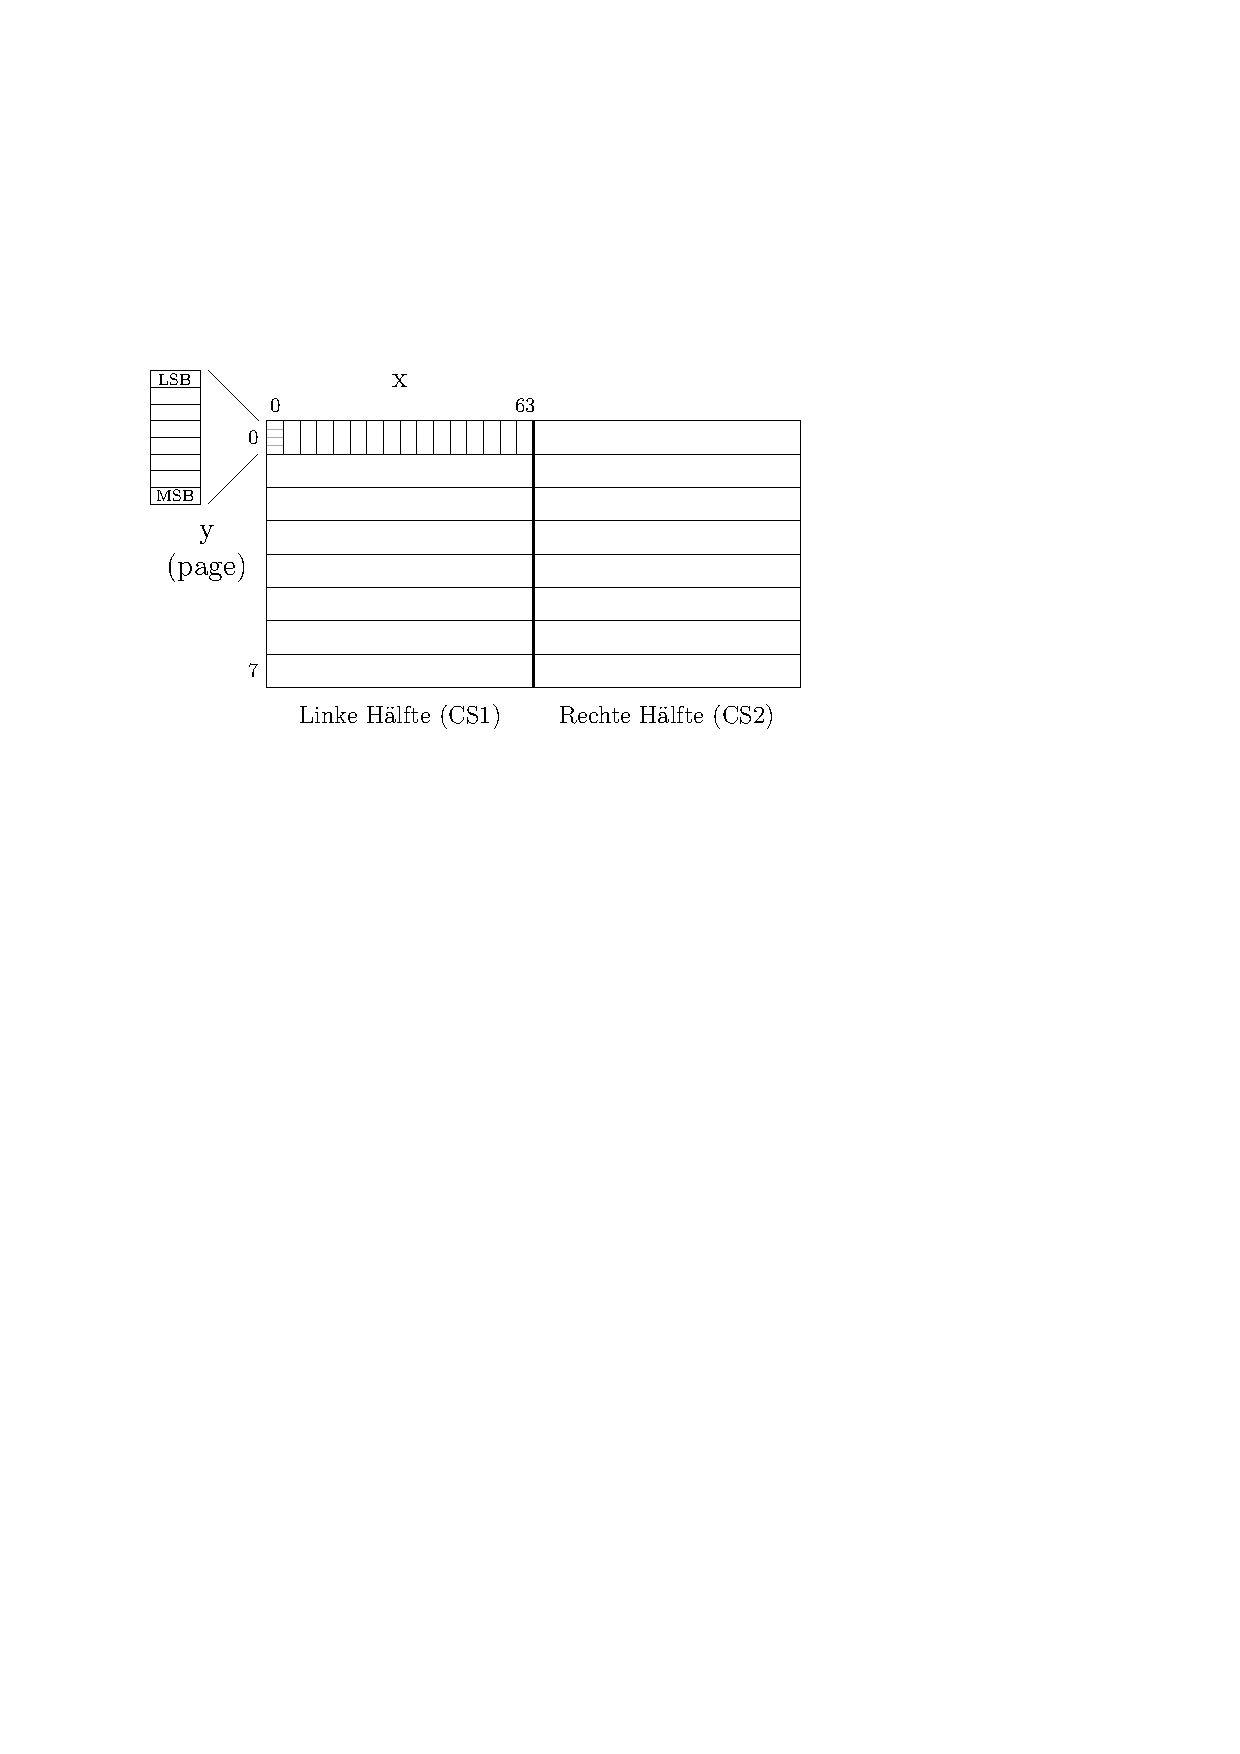
\includegraphics[width=0.6\textwidth]{figures/display_aufbau}
\end{center}

Welche Hälfte einen Befehl verarbeiten soll, wird ausgewählt, indem deren Chip-Select-Signal auf 1 gesetzt wird, das andere auf 0:
\lstinputlisting{problems/listings/display_parts.c}

\subsubsection*{Befehle senden}
Ein Befehl an das Display besteht grundsätzlich aus zwei Phasen:
\begin{enumerate}
\item Setzen der entsprechenden Pins (meist \lstinline{LCD_PIN_DI}, \lstinline{LCD_PORT_DB}).
	Eventuell selektieren der Displayhälfte über \lstinline{LCD_PIN_CS1, LCD_PIN_CS2}.

\item
Senden des \lstinline{enable}-Signals.
Setze dazu den Enable-Pin auf 1, warte kurz, setze den Pin wieder auf 0 und warte erneut kurz.
Verwende als Warteintervall die Konstante \lstinline{LCD_T}.

Es empfiehlt sich, für dieses Signal eine eigene Funktion zu schreiben (\lstinline{void lcd_sendEnable(void)}).
\end{enumerate}

\subsubsection*{Auf das Display zeichnen}
Das Vorgehen zum Zeichnen sieht in etwa wie folgt aus:
\begin{enumerate}
	\item Setzen der x-Adresse (Zeile)
	\item Setzen der y-Adresse (Spalte)
	\item Senden von 8 Bit Daten (eine \glqq{}Zelle\grqq{} von 8 Pixeln Höhe)
\end{enumerate}

\subsection{LCD manuell ansteuern}

Implementiere ein Programm, dass die linke Seite des Displays ansteuert und alle Zellen mit dem Wert AA\textsubscript{h} (10101010\textsubscript{b}) belegt, was einem sehr feinen Streifenmuster entspricht.

Der \lstinline{x}-Zähler wird nach dem Senden von Daten zum Display automatisch hochgezählt.
Somit ist es sinnvoll, beim Zeichnen zuerst über die Seiten (\lstinline{y}) zu iterieren und innerhalb dieser Schleife über die Spalten (\lstinline{x}):
\lstinputlisting{problems/listings/lcd_basics.c}

\hints{
	\item Denke daran, \lstinline{LCD_PIN_E} zu Beginn des Programms mit 0 zu initialisieren.
	\item Das Reset-Signal (\lstinline{LCD_PIN_RESET}) muss immer 1 (deaktiviert) sein.
}

\subsection{LCD Framebuffer}
Nun soll das Display wie ein Bildschirm angesteuert werden können.
Dazu wirst du einen Framebuffer verwenden, der den Bildschirminhalt repräsentiert.
In jeder Iteration wird der Framebuffer zunächst vollständig vorbereitet und dann am Stück übertragen.

Die Vorlage enthält bereits ein Array \lstinline{lcd_buffer}, das als Framebuffer fungieren soll.

Implementiere folgende Funktionen:
\lstinputlisting{problems/listings/lcd_buffer.c}

\hints{
	\item Ein Testprogramm steht bereits zur Verfügung, welches ein Schachbrettmuster auf dem Display ausgibt -- wenn deine Funktionen komplett und korrekt implementiert sind.
	\item Achte auch hier darauf, dass das Display zunächst per Befehl eingeschaltet werden muss (\emph{Display on}).
	\item Für die Funktion \lstinline{lcd_drawPixel} werden die bitweisen Operationen AND und OR sowie der Shift-Operator benötigt.
	Eine Skizze kann hier sinnvoll sein, um sich vorzustellen, wie die bitweisen Operationen arbeiten.
	\item Wenn du später bewegte Dinge visualisierst, kann es sein, dass das Display flimmert.
	Hier hilft es, entweder die Anzeige nur zu verändern, wenn sich tatsächlich etwas bewegt oder das Display vor dem Schreiben des Framebuffers aus- (\emph{Display off}) und danach wieder einzuschalten (\emph{Display on}).
}
